%Effe een titel gemaakt met geschikte logo...
\begin{titlepage} 
	\newcommand{\HRule}{\rule{\linewidth}{0.5mm}} % \Hrule is gelijk aan een een horizontale lijn met de lengte van een tekstlijn en dikte van een halve milimeter
	
	\center% Centralisatie van de elementen die volgen na deze command
	
	%------------------------------------------------
	%	Titels/subtitels
	%------------------------------------------------
	
	\textsc{\LARGE Lyceum}\\[1.5cm] % Onze school
	
	\textsc{\Large Kinematica}\\[0.5cm] % Hoofdonderwerp 
	
	\textsc{\large Fysica}\\[0.5cm] % Het vak
	
	%------------------------------------------------
	%	Titel
	%------------------------------------------------
	
	\HRule\\[0.4cm] %\\[<lengte>] is afstand tussen de hoofdtitel en lijn(Hrule)
	
	{\huge\bfseries Valbeweging van de bal}\\[0.4cm] % Hoofdtitel
	
	\HRule\\[1.5cm]
	
	%------------------------------------------------
	%	Schrijvers
	%------------------------------------------------
	
	\begin{minipage}{0.4\textwidth}
		\begin{flushleft} %De tekst begint links
			\large
			\textit{Auteurs}\\
			Fidon \textsc{Namani}\\
			Jorn \textsc{Smit} % Ik 
		\end{flushleft}
	\end{minipage}
	 % Dit golfje geeft aan dat deze twee minipagina's nooit onder elkaar mogen komen te staan.
	\begin{minipage}{0.4\textwidth}
		\begin{flushright} %De tekst begint rechts
			\large
			\textit{Beoordeler}\\
			E.\textsc{Zijlstra} % Jij
		\end{flushright}
	\end{minipage}


	
	%------------------------------------------------
	%	Datum
	%------------------------------------------------
	
	\vfill\vfill\vfill % De datumverschijning is 3/4 lengte van top van papier geplaatst.
	
	{\large\today} % Datum
	
	%------------------------------------------------
	%	Logo
	%------------------------------------------------
	
	\vfill\vfill
	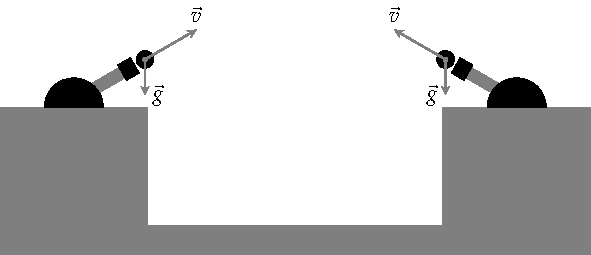
\includegraphics[width=0.75\textwidth]{Cannon.pdf}\\[1cm] % Ons fysica logootje
	 
	
	\vfill %De datum wordt voor de zekerheid nog 1/4 deel van de bodem van papier naar boven geduwd
\end{titlepage}
%%
